%%%%%%%%%%%%%%%%%%%%%%%%%%%%%%%%%%%%%%%%%
% Arsclassica Article
% LaTeX Template
% Version 1.1 (10/6/14)
%
% This template has been downloaded from:
% http://www.LaTeXTemplates.com
%
% Original author:
% Lorenzo Pantieri (http://www.lorenzopantieri.net) with extensive modifications by:
% Vel (vel@latextemplates.com)
%
% License:
% CC BY-NC-SA 3.0 (http://creativecommons.org/licenses/by-nc-sa/3.0/)
%
%%%%%%%%%%%%%%%%%%%%%%%%%%%%%%%%%%%%%%%%%

%----------------------------------------------------------------------------------------
%	PACKAGES AND OTHER DOCUMENT CONFIGURATIONS
%----------------------------------------------------------------------------------------

\documentclass[
10pt, % Main document font size
a4paper, % Paper type, use 'letterpaper' for US Letter paper
oneside, % One page layout (no page indentation)
%twoside, % Two page layout (page indentation for binding and different headers)
headinclude,footinclude, % Extra spacing for the header and footer
BCOR5mm, % Binding correction
]{scrartcl}

%%%%%%%%%%%%%%%%%%%%%%%%%%%%%%%%%%%%%%%%%
% Arsclassica Article
% Structure Specification File
%
% This file has been downloaded from:
% http://www.LaTeXTemplates.com
%
% Original author:
% Lorenzo Pantieri (http://www.lorenzopantieri.net) with extensive modifications by:
% Vel (vel@latextemplates.com)
%
% License:
% CC BY-NC-SA 3.0 (http://creativecommons.org/licenses/by-nc-sa/3.0/)
%
%%%%%%%%%%%%%%%%%%%%%%%%%%%%%%%%%%%%%%%%%

%----------------------------------------------------------------------------------------
%	REQUIRED PACKAGES
%----------------------------------------------------------------------------------------

\usepackage[
nochapters, % Turn off chapters since this is an article        
beramono, % Use the Bera Mono font for monospaced text (\texttt)
eulermath,% Use the Euler font for mathematics
pdfspacing, % Makes use of pdftex’ letter spacing capabilities via the microtype package
dottedtoc % Dotted lines leading to the page numbers in the table of contents
]{classicthesis} % The layout is based on the Classic Thesis style

\usepackage{arsclassica} % Modifies the Classic Thesis package

\usepackage[T1]{fontenc} % Use 8-bit encoding that has 256 glyphs

\usepackage[utf8]{inputenc} % Required for including letters with accents

\usepackage{graphicx} % Required for including images
\graphicspath{{Figures/}} % Set the default folder for images

\usepackage{enumitem} % Required for manipulating the whitespace between and within lists

\usepackage{lipsum} % Used for inserting dummy 'Lorem ipsum' text into the template

\usepackage{subfig} % Required for creating figures with multiple parts (subfigures)

\usepackage{amsmath,amssymb,amsthm} % For including math equations, theorems, symbols, etc

\usepackage{varioref} % More descriptive referencing

%----------------------------------------------------------------------------------------
%	THEOREM STYLES
%---------------------------------------------------------------------------------------

\theoremstyle{definition} % Define theorem styles here based on the definition style (used for definitions and examples)
\newtheorem{definition}{Definition}

\theoremstyle{plain} % Define theorem styles here based on the plain style (used for theorems, lemmas, propositions)
\newtheorem{theorem}{Theorem}

\theoremstyle{remark} % Define theorem styles here based on the remark style (used for remarks and notes)

%----------------------------------------------------------------------------------------
%	HYPERLINKS
%---------------------------------------------------------------------------------------

\hypersetup{
%draft, % Uncomment to remove all links (useful for printing in black and white)
colorlinks=true, breaklinks=true, bookmarks=true,bookmarksnumbered,
urlcolor=webbrown, linkcolor=RoyalBlue, citecolor=webgreen, % Link colors
pdftitle={}, % PDF title
pdfauthor={\textcopyright}, % PDF Author
pdfsubject={}, % PDF Subject
pdfkeywords={}, % PDF Keywords
pdfcreator={pdfLaTeX}, % PDF Creator
pdfproducer={LaTeX with hyperref and ClassicThesis} % PDF producer
} % Include the structure.tex file which specified the document structure and layout

\hyphenation{Fortran hy-phen-ation} % Specify custom hyphenation points in words with dashes where you would like hyphenation to occur, or alternatively, don't put any dashes in a word to stop hyphenation altogether
\usepackage{pgfgantt}
\usepackage{lipsum}
\usepackage{float}
\usepackage{caption}
\usepackage{ragged2e}


%----------------------------------------------------------------------------------------
%	TITLE AND AUTHOR(S)
%----------------------------------------------------------------------------------------

\title{\normalfont\spacedallcaps{Data Analytics Coursework: Predict the 2017 NCAA Basketball Tournament}} % The article title
\author{\spacedlowsmallcaps{Ivaylo Snezhanov Shalev, Ziqi Zhao, Yuan-Yi Chang}} % The article author(s) - author affiliations need to be specified in the AUTHOR AFFILIATIONS block

\date{} % An optional date to appear under the author(s)

%----------------------------------------------------------------------------------------

\begin{document}

%----------------------------------------------------------------------------------------
%	HEADERS
%----------------------------------------------------------------------------------------

\renewcommand{\sectionmark}[1]{\markright{\spacedlowsmallcaps{#1}}} % The header for all pages (oneside) or for even pages (twoside)
%\renewcommand{\subsectionmark}[1]{\markright{\thesubsection~#1}} % Uncomment when using the twoside option - this modifies the header on odd pages
\lehead{\mbox{\llap{\small\thepage\kern1em\color{halfgray} \vline}\color{halfgray}\hspace{0.5em}\rightmark\hfil}} % The header style

\pagestyle{scrheadings} % Enable the headers specified in this block

%----------------------------------------------------------------------------------------
%	TABLE OF CONTENTS & LISTS OF FIGURES AND TABLES
%----------------------------------------------------------------------------------------

\maketitle % Print the title/author/date block

\setcounter{tocdepth}{2} % Set the depth of the table of contents to show sections and subsections only

\tableofcontents % Print the table of contents

%\listoffigures % Print the list of figures

%\listoftables % Print the list of tables

%----------------------------------------------------------------------------------------
%	ABSTRACT
%----------------------------------------------------------------------------------------

%\section*{Abstract} % This section will not appear in the table of contents due to the star (\section*)

%\lipsum[1] % Dummy text

%----------------------------------------------------------------------------------------
%	AUTHOR AFFILIATIONS
%----------------------------------------------------------------------------------------

%{\let\thefootnote\relax\footnotetext{* \textit{Department of Biology, University of Examples, London, United Kingdom}}}

%{\let\thefootnote\relax\footnotetext{\textsuperscript{1} \textit{Department of Chemistry, University of Examples, London, United Kingdom}}}

%----------------------------------------------------------------------------------------

\newpage % Start the article content on the second page, remove this if you have a longer abstract that goes onto the second page

%----------------------------------------------------------------------------------------
%	Problem description
%----------------------------------------------------------------------------------------

\section{Problem Description}
The National Collegiate Athletic Association(NCAA) Basketball Tournament is not only a competition but also given an opportunity for college players to enter NBA, the world's most well-known professional Basketball league. We are given the historical data from 1985 to 2016 in regular season and try to predict every matchups in 2017 NCAA.

%----------------------------------------------------------------------------------------
%	Dataset
%----------------------------------------------------------------------------------------

\section{Dataset}
After analysing data sets from different sources we decided to use the \textit{KenPom} statistical data of all US basketball teams for the past 15 years (from 2002). As helping dataset of the teams playing this year we used the \textit{Kaggle's} dataset. \cite{kaggle,kenpom}
\subsection{Data Collection}
\textit{Kaggle} has provided well organised data simply in \textbf{csv} file format, therefore you don't have to collect the data by ourself. However, the \textit{KenPom} statistical data are listed only on the website. We have written a web crawler to fetch all the data from \textit{KenPom} by using \textit{Python} package: \textbf{scrapy} and \textbf{BeatifulSoup}. In order to match the data from \textit{Kaggle} and \textit{KenPom} in data cleaning stage, we make consistent with \textbf{\textit{Team Name}} of both data. Unfortunately, there are some mismatch so that we have to check the \textbf{\textit{Team Name}} one by one.
\subsection{Features Description}
The KenPom statistical data includes the years of 2002 until 2016 and includes 10 features. This data is collected and calculated based on the idea of the four factor concept from Dean Oliver.
Oliver believes four factors determine why a team wins or loses. The four factors are:
\begin{enumerate}
\item Shooting
\item Avoiding turnovers
\item Offensive rebounding
\item Getting to the foul line
\end{enumerate}
A team is measured both offensively and defensively on these four factors.
\subsubsection{Number of wins and losses (W-L)}
This is aggregative value of the total games won (W) and lost (L) for the team, for the specific season (year). As we are trying to predict if team A will win against team B for the upcoming tournament (season) we can't use this feature as we will not know the wins and loses for the tested new season.
\subsubsection{Adjusted Efficiency Margin (AdjEM)}
This is the difference between a team’s offensive and defensive efficiency.
\[AdjEM = AdjOE - AdjDE\]
AdjEM is used to rate teams. It was introduced by KenPom website prior to the 2016-2017 season. Prior to this metric, ratings were built on log5 and the Pythagorean expectation.

The adjusted efficiency margin shows the number of points a team would be expected to outscore the average Division-I team over 100 possessions without adjusting for location of the game.
For example, in 2015-2016, if Villanova played the average Division-I team on a neutral court, on average, Villanova would win a 100-possession game by about 32 points.
Villanova's AdjOE is 121.7 and AdjDE is 89.7.\[AdjEM = 121.7 - 89.7 = 32\] AdjEM is used because it's simpler and it's a linear measure.
The Pythagorean expectation, from the mind of Bill James, originated from baseball. It estimates how many games a team should have won based on the amount of runs it scored or allowed.
It applied to college basketball by giving you a team's expected winning percentage against the average Division-I team.\[Pyth = (AdjOE^{11.5}) / (AdjOE^{11.5} + AdjDE^{11.5})\]
It's clear the Pythagorean expectation is complicated. AdjEM is subtraction. That's it. A team's offensive efficiency minus its defensive efficiency.
The difference when comparing teams using AdjEM versus log5 or the Pythagorean expectation is important too. The Pythagorean expectation for one team could be .96 and for another could be .93. The difference of .3 there is not the same as comparing teams with a .70 and .67 expected winning percentage because of the team's strength. It's murky.
KenPom describes AdjEM as a linear measure giving the example of a team with a +31 AdjEM and a team with a +28 AdjEM the same as the difference between +4 and +1. It's more clear.\cite{adjem}

\subsubsection{Adjusted offensive efficiency (AdjO)}
A team's offensive efficiency is the amount of points it scores per 100 offensive possessions.
\[OE = (Points scored * 100) / Possessions\]
A team's pace is determined by how they like to play and how their opponents like to play. This is the reason efficiency numbers need to be adjusted. It accounts for competition or how a team and their opponents want to play.

\subsubsection{Adjusted defensive efficiency (AdjD)}
A team's defensive efficiency is the amount of points it allows per 100 defensive possessions.
\[DE = (Points allowed * 100) / Possessions\]

\subsubsection{Adjusted tempo (AdjT)}
Possessions per 40 minutes. In every game, each team wants to play at a certain pace. Adjusted tempo tries to tell you the pace each team wants to play. It's an estimate of the pace a team would have against the team that wants to play at an average Division-I tempo.

\subsubsection{Luck rating (Luck)}
Luck doesn't factor into a team's rating. It's a metric that compares a team's record to what they deserved based on their game-by-game efficiency.
If a team is involved in a lot of close games, it shouldn't win or lose all of them. If a team wins all of the close games, they're viewed as a lucky. An unlucky team would lose all of their close games.
Luck is measured using Dean Oliver's correlated Gaussian method.
If this sounds complicated, it definitely is.
Oliver explains it as something similar to a bell curve.
\begin{equation}
Win\% = \mathit{NORM}\left [ \frac{\left (Rtg-Opp.Rtg \right )}{\mathit{SD}\left ( Rating Difference \right )} \right ]
\end{equation}
\begin{equation}
\begin{split}
\mathit{SD}\left(Rating Difference\right) & = \mathit{SD}\left(Rtg - Opp.Rtg\right)  \\
							& = \mathit{SQRT}\left(\mathit{Var}\left(Rtg\right)+\mathit{Var}\left(Opp.Rtg\right) - 2*\mathit{Cov}\left(Rtg,Opp.Rtg\right)\right)
\end{split}
\end{equation}
The components:
\begin{enumerate}
\item Rtg: points scored per 100 possessions (offensive rating)
\item Opp.Rtg: points allowed per 100 possessions (defensive rating)
\item \textit{SD}: statistical standard deviation of quantity in parentheses ()
\item \textit{Var}: statistical variance of quantity in parentheses ()
\item \textit{Cov}: statistical covariance of quantities in parentheses ()
\end{enumerate}

Luck tells you the difference between expected winning percentage and its actual winning percentage.
Luck doesn't use Pythagorean Winning Percentage (Pyth) as the expected winning percentage. Pyth is calculated by a team's offensive and defensive efficiencies.
The correlated Gaussian method uses the distribution of a team's game efficiencies to determine the expected winning percentage. It includes both the average margin of victory and the variation in a team's margin of victory.
This method takes into account that the majority or teams play to the level of their competition.\cite{luck}

%\begin{description}
%\item[Example]
%In 2015-2016, Hampton was viewed as the second luckiest team in Division-I.
%Hampton was 21-11. It's actual winning percentage was .656.
%Using the correlated Gaussian method, Hampton's expect winning percentage was .499.
%Hampton's actual winning percentage is .157 points higher than its expected. This translates into roughly 5 wins that are attributed to luck.
%If you take a glance at Hampton's results, it played 3 overtime games and one double-overtime game. It won all 4 of these contests, which can be viewed as lucky.
%In comparison, the 2015-2016 Clemson Tigers finished 17-14. Clemson was ranked 339th out of 351 teams in luck.
%Clemson's actual winning percentage was .548.
%It's expected winning percentage using Oliver's method was .643.
%This is -0.095 points lower than expected. This means almost 3 losses were attributed to luck.
%Taking a look at Clemson's game-by-game results, you'll find 10 losses by a 7 points or less. This can be seen as unlucky.
%Remember luck doesn't factor into ratings
%Luck isn't used when rating a team. It gives you an idea on how a team performs in close game and how it plays to its competition.
%A very lucky team will likely be rated lower by KenPom.
%Where an extremely unlucky team could be rated higher.
%Using our example above, Hampton (lucky) was 229th in the final 2015-2016 KenPom ratings.
%While Clemson (unlucky) was 48th in the final 2015-2016 KenPom ratings.\cite{luck}
%\end{description}

\subsubsection{Strength of schedule (SOS)}
A team's strength of schedule is made up of 3 components:
\begin{description}
\item[AdjEM] The overall strength of schedule of a team.
\item[AdjO] Opponent's average adjusted offensive efficiency.
\item [AdjD] Opponent's average adjusted defensive efficiency.
\end{description}
AdjEM for strength of schedule is calculated:
\[AdjEM of SOS = AdjO - AdjD\]
Prior to the 2016-17 season, KenPom started using AdjEM for ratings and strength of schedule instead of the Pythagorean expectation and log5.
Another change is now KenPom is using Jeff Sagarin's WIN50 Method.

Sagarin's WIN50 method shows the strength of a team that would be expected to win half its games against the team's schedule. It compares all teams on the same scale and reduces the impact of outliers.

The previous method used by KenPom measured a team's strength of schedule by the average of its opponents' rating. This means outliers like playing the 350th or 351st team would have a negative impact on a team's SOS.

The WIN50 method doesn't put too much emphasis on the quality of bad opponents a team plays. It's more fair than previous methods.

Outside of factoring into a team's rating or predicting how it will perform, strength of schedule can be used to rate different conferences as a whole.\cite{sos}

\subsubsection{Adjusted Efficiency Margin (SOS AdjEM)}
The Adjusted Efficiency Margin, but just durring the season.

\subsubsection{Average AdjOE of opposing offenses (SOS OppO)}
The Adjusted Offence Efficiency just durring the season.

\subsubsection{Average AdjDE of opposing defenses (SOS OppD)}
The Adjusted Defence Efficiency just driving the season.

\subsubsection{Non-conference strength of schedule (NCSOS)}
A team does have some control over its schedule. It can choose or agree to its non-conference schedule.
The non-conference strength of schedule uses the 3 components only for this portion of the schedule. It doesn't include post season or conference games.

\begin{enumerate}
\item NCSOS AdjEM is the non-conference strength of schedule of a team. It's calulated using NCSOS AdjO and NCSOS AjdD:
\[NCSOS AdjEM = NCSOS AdjO - NCSOS AjdD\]
\end{enumerate}

\subsection{Data Cleaning}
We obtain two attributes \textbf{Team1\_ID} and \textbf{Team2\_ID} from the team id of winning and losing team, keeping \textbf{Team1\_ID} is less than \textbf{Team2\_ID} in each matchup data from Kaggle, and create a new attribute \textbf{W/L} denoting 1 if team 1 is the winning team, 0 if team 2 is the wining team. Then merging two dataset \{Kaggle, KenPom\} by mapping statistical data to each matchup data to obtain the final data matrix which the row is the matchup had been played and the column is the feature. We apply left join when merging both dataset, so it would have some missing data if the team doesn't have the statistical data from KenPom.

%----------------------------------------------------------------------------------------
%	Exploration
%----------------------------------------------------------------------------------------

\section{Exploration}
\subsection{Finding sources of data}
\subsubsection{Kaggle}
As the idea of this project came from the famous data science competitions website Kaggle (kaggle.com) we started by looking the data provided there. The data there is collected and uploaded by the different teams. The most interesting for us files available there were:
\begin{itemize}
\item Teams.csv: contains all 365 teams in USA possible to play in the tournament. Each team has a 4-digit long ID number, which is used as a key through all files.
\item RegularSeasonCompactResults.csv: contains the results of previous year's tournaments (from 1985 until 2016). Which year, which team played with which team and their score and few more details.
\item SampleSubmission.csv: the file containing the predictions for this year's tournament. This file contains the ID’s only of the 68 teams playing this season, with all possible matches between them (2 278) and the outcome prediction as a floating point number between 0 and 1 (showing the probability that the first team wins over the second).
\end{itemize}
There are more files available containing detailed information about the teams and seasons for the past 13 years, but as it will be explained later on, we decided to not use them.

\subsubsection{Kenpom}

\subsection{Final choice of data}
By using this already verified, calculated and proved rating data as a training data for the model we can prove that there is a relation between the rating of a team and its actual win or loss in each season.
The data from Kenpom shows the rating of a team for each season. The Kaggle’s data give us information for each season which team won during the tournament and which lost. Combining these two together and using this a training data for the model will allow us to create a more precise prediction for the outcomes of the current season.

\subsection{Exploration}
\subsubsection{Kaggle}
The exploration started by getting to know the data from Kaggle using Jupyter Notebook (Python 2.7 - Anaconda) and the libraries numpy and pandas we’ve loaded the CSV files into data frames which were used later on in the manipulations.
As simple preview of the data we printed the first and last few rows using the head and tail commands in almost every script. Another useful command was shape, which showed us the number of rows and columns in the dataframe.
To see the teams that participated most in the tournament during the years we used a group by and counted how many occurrences a team had in the RegularSeasonCompactResults file. After that using the join command with the Teams file we joined the team names and visualised the top 20 in descending order of their occurrences.
Using the SampleSubmission file and the Teams file we managed to create a list of the 68 teams playing this season (merge command – inner join) with their Ids and Names (CODE: DA - NCAA - Get Teams 2017.ipynb).
\subsubsection{Kenpom}
After the extraction of the data from the website and it’s merged with the Kaggle data we started exploring the created dataset.
We’ve checked the distribution of the data (using histograms) and the relation of the features with the target. We used a free tool called Weka created for data analysis, exploration, visualisation and building of models. This exploration helped us to see if there are any outliers, missing data and anomalies in the data. The relation diagrams help us see if some of the features have more outstanding relation with the target.

\begin{figure}[H]
\caption{Histogram - Python (matplot library)}
  \centering
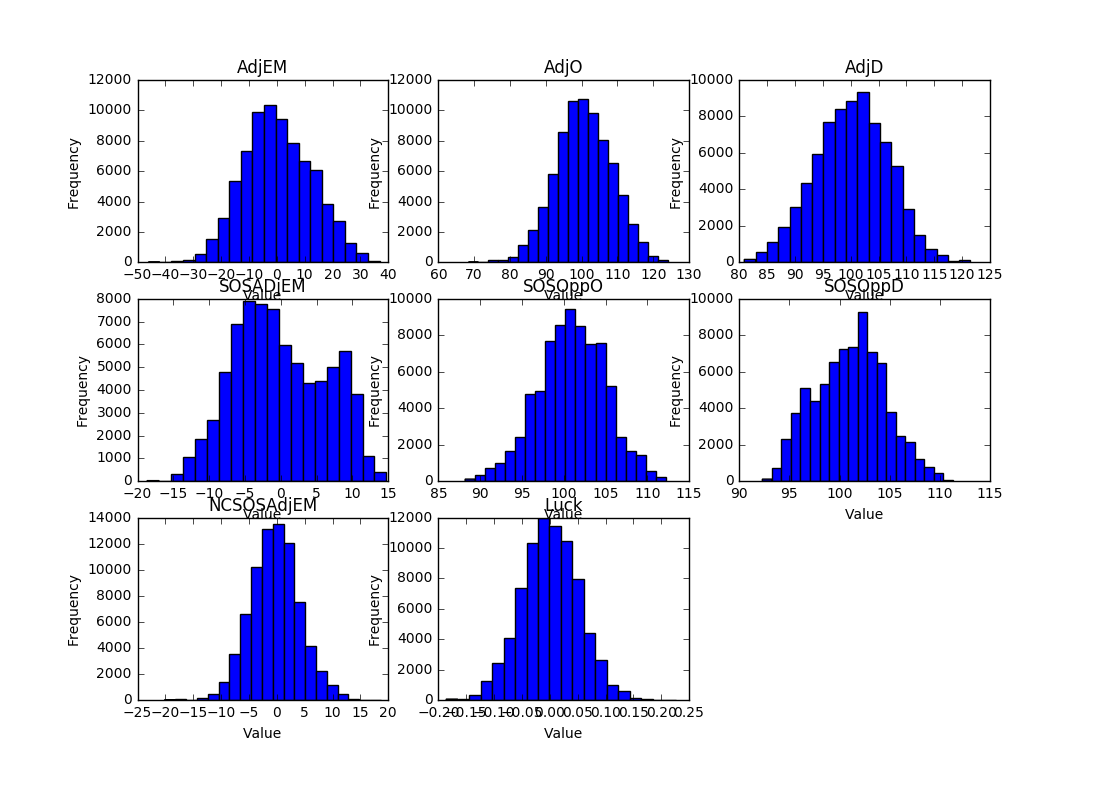
\includegraphics[width=\textwidth]{Histograms}
\end{figure}

\begin{figure}[H]
\caption{Weka histogram}
  \centering
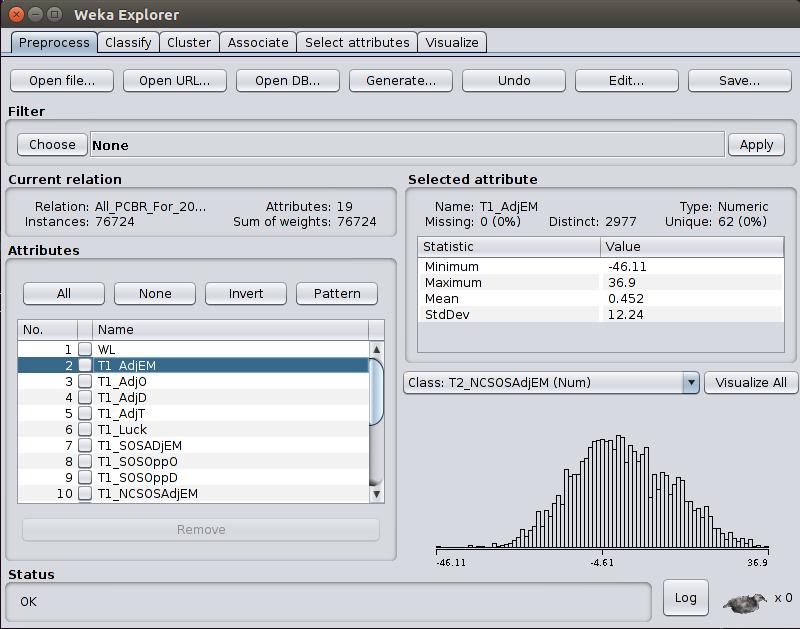
\includegraphics[width=\textwidth]{Weka_Histogram1.png}
\end{figure}

\begin{figure}[H]
\caption{Weka histogram}
  \centering
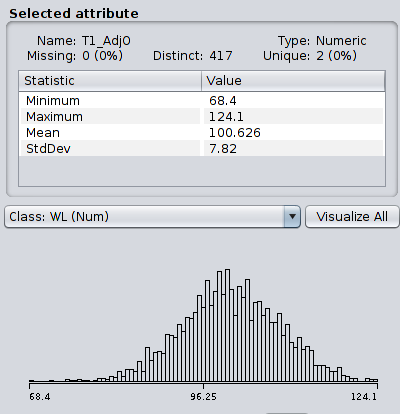
\includegraphics[width=\textwidth]{Weka_Histogram2.png}
\end{figure}

\begin{figure}[H]
\caption{Weka histogram}
  \centering
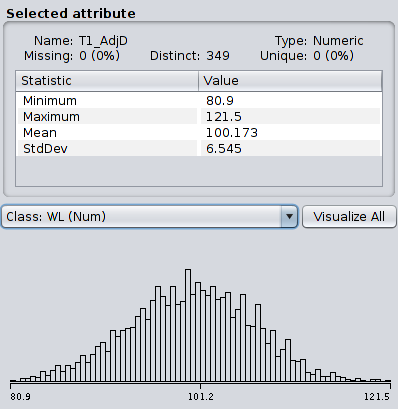
\includegraphics[width=\textwidth]{Weka_Histogram3.png}
\end{figure}

\begin{figure}[H]
\caption{Weka histogram}
  \centering
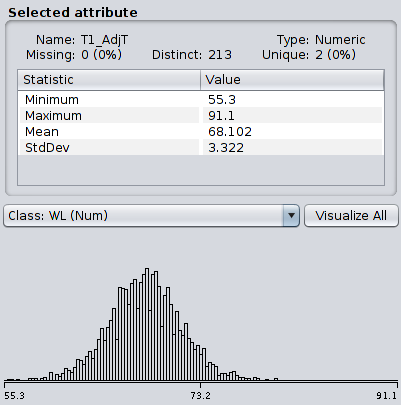
\includegraphics[width=\textwidth]{Weka_Histogram4.png}
\end{figure}

As a result, we didn’t notice any large outliers or any missing data. The distribution was in the expected normal distribution shape for most of the features.

\begin{figure}[H]
\caption{Correcation of the features with the target (WL)}
  \centering
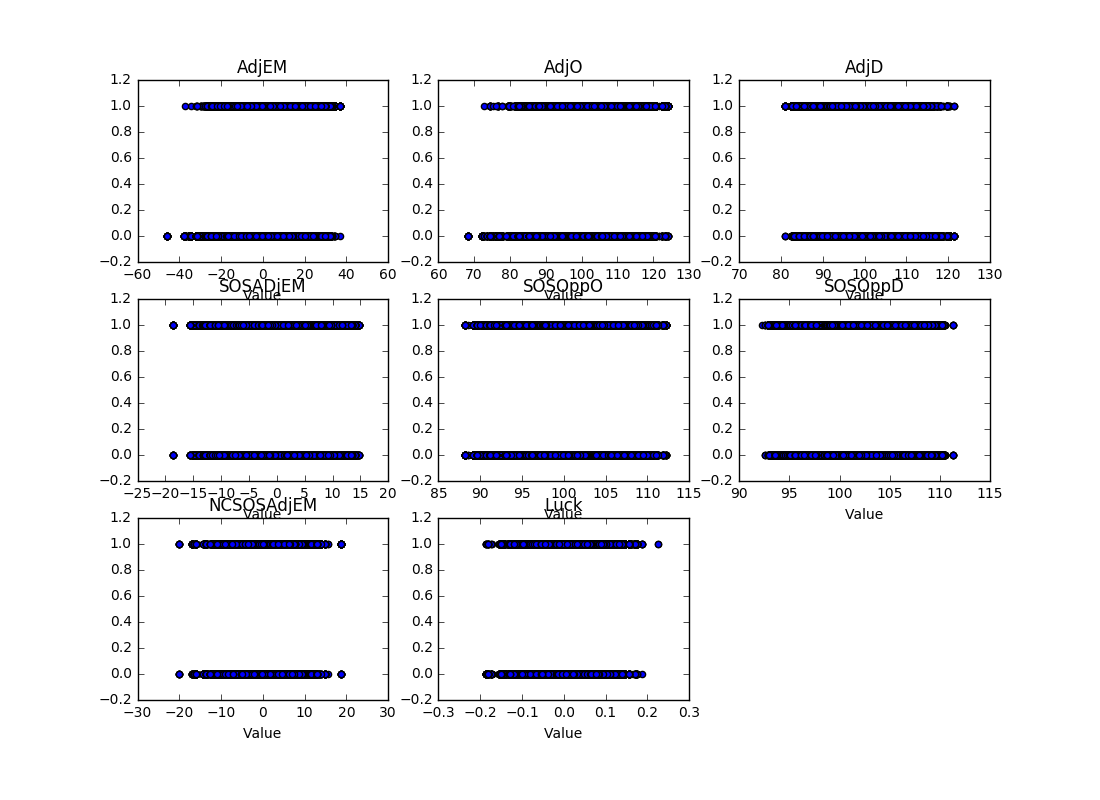
\includegraphics[width=\textwidth]{Correlation1}
\end{figure}

\begin{figure}[H]
\caption{Scatter diagrams – Weka – Correlation of Luck with WL}
  \centering
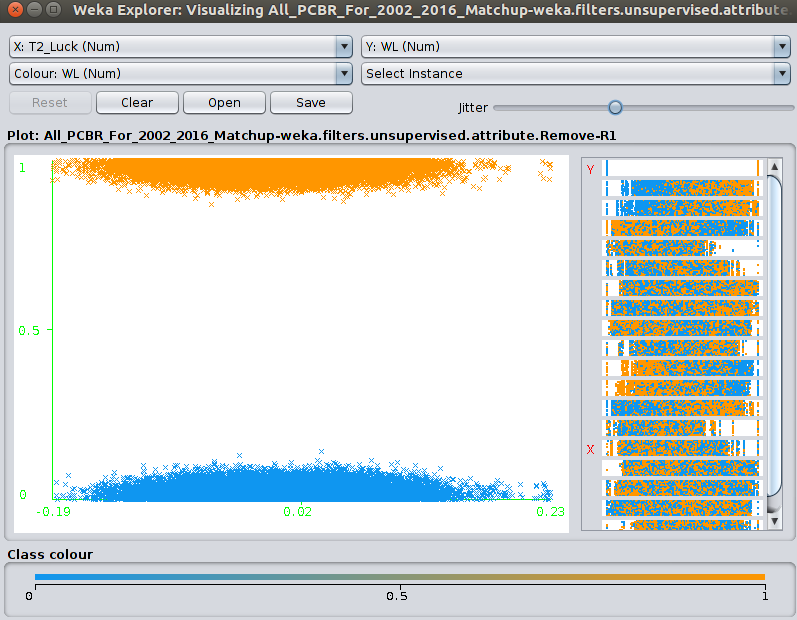
\includegraphics[width=\textwidth]{Weka_Correlation_Luck_WL}
\end{figure}

The correlation diagrams show some expected results. Mainly that the distribution is almost equal between the features and the target. It doesn’t matter if the offence or defence is high. Both have equal chance of winning or losing the game. Correlation of features between themselves and target as colour (WL – 0 – yellow, 1 – blue). The yellow is drawn on top of the blue.
\begin{figure}[H]
  \centering
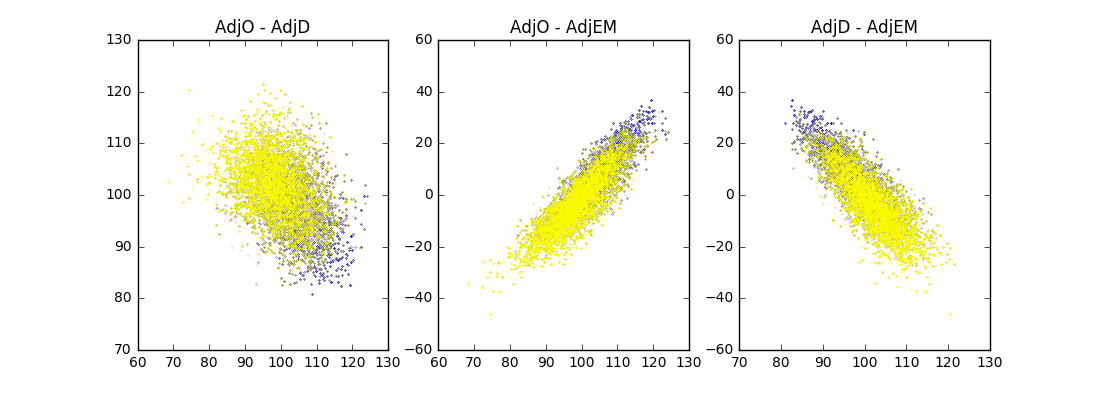
\includegraphics[width=\textwidth]{Correlation2}
\end{figure}
When comparing both offence and defence and plotting the win/loose with different colour, we can see a small trend that the winning teams have higher offence and lower defence. The same with EM (margin) the higher the margin the higher the chance for win.
\begin{figure}[H]
  \centering
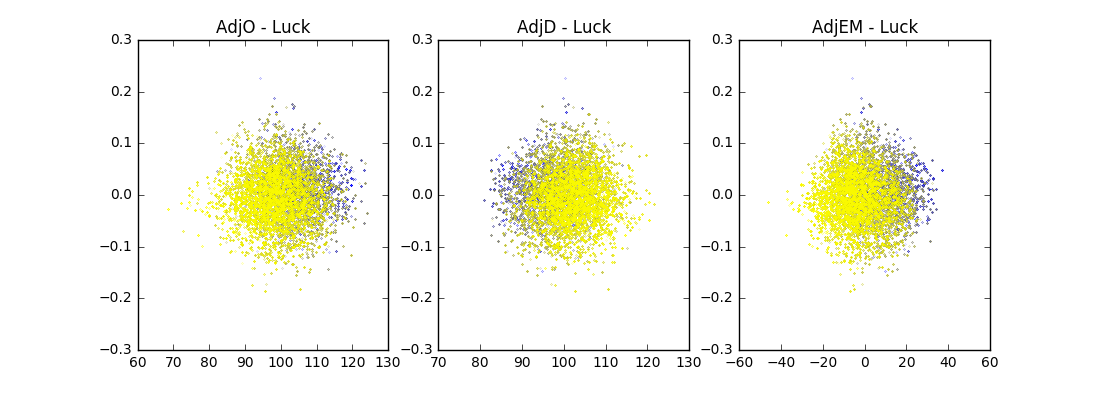
\includegraphics[width=\textwidth]{Correlation3}
\end{figure}
On the other side the Luck also helps a bit (higher Luck bigger chance for win), but the graphics which show the relation between Luck and AdjO and AdjD again confirm that higher offence and lower offence are more typical for a winning team.
\begin{figure}[H]
  \centering
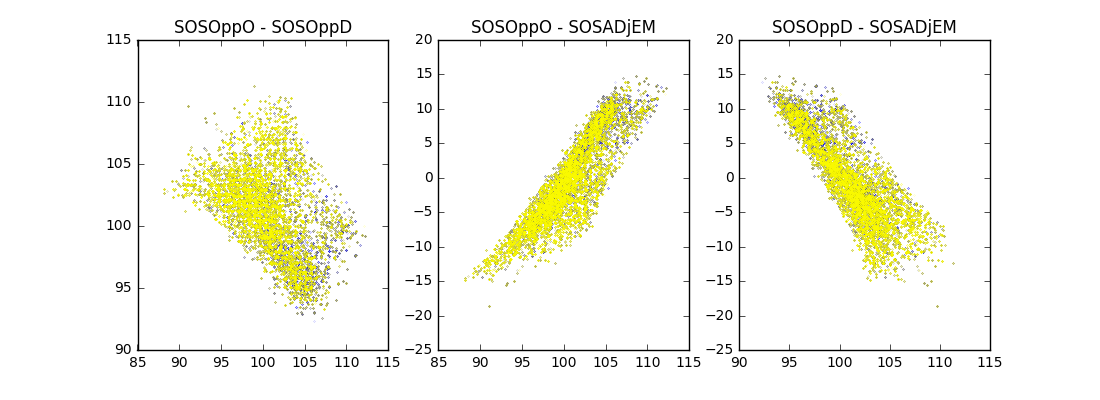
\includegraphics[width=\textwidth]{Correlation4}
\end{figure}
Looking into SOS features we see similar relations with linear borders as of the way SOS is calculated there is a linear rule between the offence and defence.
\begin{figure}[H]
  \centering
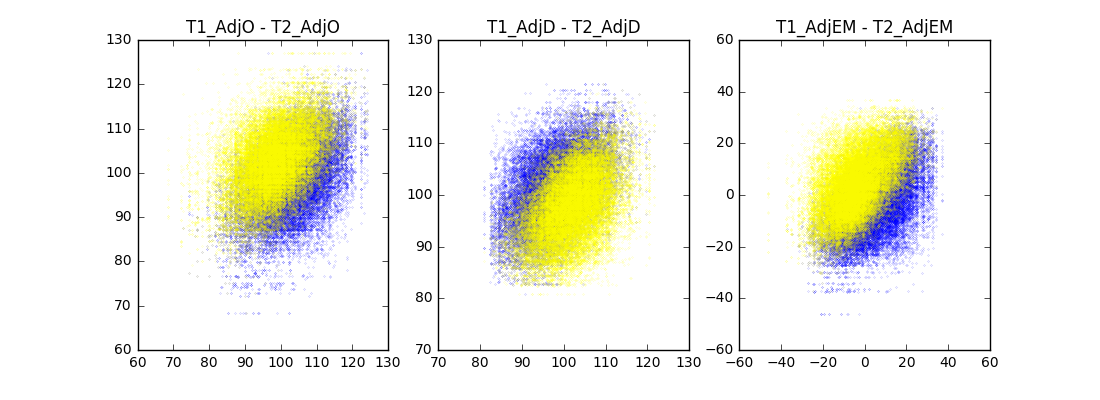
\includegraphics[width=\textwidth]{Correlation5}
\end{figure}
The last 3 diagrams show correlation between the features of team 1 with same feature of team 2. As the target (WL) shows: 1- team 1 won against team 2 and 0 – team 1 lost against team 2 we can see the expected correlation that when the offence is higher (but not too high) for team 1 and the offence for team 2 is lower (but not too low) there is higher chance for team 1 to win (WL = 1). The same for EM and the other way for defence – the lower the defence of team 1 and higher defence for team 2, the higher the chances of team 1 to win. The area where the blue color is more intense is the area of win – it’s perfect balance between offence and defence.


%----------------------------------------------------------------------------------------
%	Analysis
%----------------------------------------------------------------------------------------

\section{Analysis}
\subsection{Feature}
Features are the input of model, which are cleaned from original data and selected as many combinations to optimise the model. As shown in Table \ref{my-label}
\begin{table}[H]
\centering
\caption{List of features}
\label{my-label}
\begin{tabular}{|l|l|}
\hline
\textbf{Variable} & \textbf{Description} \\ \hline
X1 & T1\_AdjEM \\ \hline
X2 & T1\_AdjO \\ \hline
X3 & T1\_AdjD \\ \hline
X4 & T1\_AdjT \\ \hline
X5 & T1\_Luck \\ \hline
X6 & T1\_SOSADjEM \\ \hline
X7 & T1\_SOSOppO \\ \hline
X8 & T1\_SOSOppD \\ \hline
X9 & T1\_NCSOSAdjEM \\ \hline
X10 & T2\_AdjEM \\ \hline
X11 & T2\_AdjO \\ \hline
X12 & T2\_AdjD \\ \hline
X13 & T2\_AdjT \\ \hline
X14 & T2\_Luck \\ \hline
X15 & T2\_SOSAdjEM \\ \hline
X16 & T2\_SOSOppO \\ \hline
X17 & T2\_SOSOppD \\ \hline
X18 & T2\_NCSOSAdjEM \\ \hline
\end{tabular}
\end{table}
\subsection{Model Selection}
\subsubsection{Logistic Regression}
\paragraph{Introduction}
Logistic regression is a regression model where we could take this model to solve binary classification problem easily. However, the original model is mapped into a sigmoid function which the domain is located in \{0, 1\}, a great representation for probability.  
\paragraph{Implementation and Optimisation of Model}
In logistic regression model, there is a significant factor: \textbf{penalty} which is a parameter we could tune in validation stage. L1-norm is also known as least absolute deviation, least absolute error. It is basically minimising the sum of the absolute differences between the target value and the estimated values. 
\begin{equation}
S = \sum_{i=1}^{n}\left | y_{i}-f(x_{i}) \right |
\end{equation}
L2-norm is also known as least square error. It is basically minimising the sum of the square of the differences between the target value and the estimated values.
\begin{equation}
S = \sum_{i=1}^{n}\left ( y_{i}-f(x_{i}) \right )^{2}
\end{equation}
\subsubsection{Neural Network}
\paragraph{Introduction}
Neural network is an information processing model that bases on a large amount of artificial neurons in various structures. Inspired by the features that biological nerves work, a general neural network consist of interconnected neurons and layers. Neurons are the units that can receive data, make computations, and give outputs. Layers are the collections of neurons, where neurons can link with those neurons located on different layers but not those on same layers. With different function of connection and diverse structure of layers, neural networks are widely used in the scenarios that people obtain massive data but can not capture the rules or patterns behind data, such as Big Data Processing or Computer Vision.\cite{ann}

\paragraph{Implementation and Optimisation of Model}
Competition prediction based on neural network model is one of the main methods in this project. Considering efficiency on limited hardware and feasibility in specified time, we chose Keras as machine learning library to build our neural network, and use Theano as backend for Keras to make graph calculations and analysis.

To optimise the model and further get the best prediction accuracy, we examine the prediction performance of neural network in different inputs, parameters and layers. In this section, the model is tested under various selection of features, activation function, batch size, optimiser and number of layers, is revealed as follows.

\begin{enumerate}
\item Feature: Features are the input of model, which are cleaned from original data and selected as many combinations to optimise the model.
\item Activation Function: Sigmoid and ReLU are two classical and popular activation function in neural network. Considering that they have no inflection point and are easy to make binary classification, this two function are applied and tested in this project.

ReLU is defined as:
\begin{equation}
f(x) = max(0,x)
\end{equation}
\begin{figure}[H]
  \caption{ReLU}
  \centering
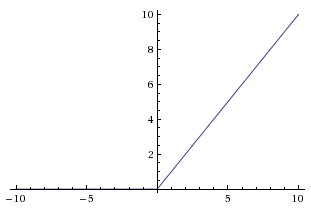
\includegraphics[width=\textwidth]{relu-figure}
\end{figure}
Sigmoid is defined as:
\begin{equation}
S(t) = \frac{1}{1+e^{-t}}
\end{equation}
\begin{figure}[H]
  \caption{Sigmoid function.}
  \centering
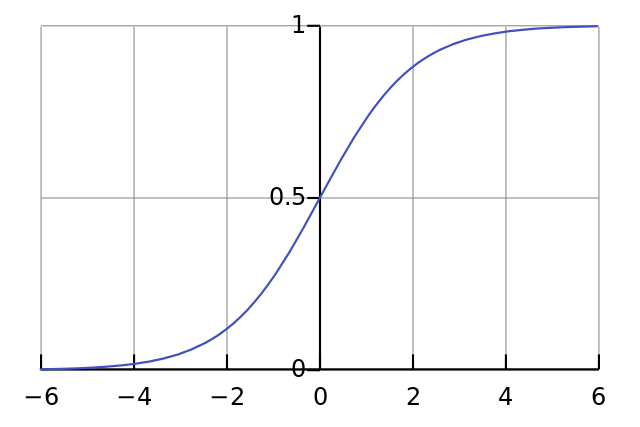
\includegraphics[width=\textwidth]{sigmoid}
\end{figure}
\item Batch Size: Batch size is the number of data to be calculated at one time. Batch size can affect the speed of convergence and performance of optimised point.
\item Optimiser is entries that regularise and modify the target function to make it reach a good convergence point within reasonable time.
\item Number of Layers (Fully Connected layers): Number of layers has affection on efficiency of feature capturing and speed of training.
\end{enumerate}

\subsection{Cross Validation}
\subsubsection{K-Fold Cross Validation}
In our analysis, we choose 10-fold cross validation to split our training data and validation data.
\subsubsection{Proposed Cross Validation}
We propose a domain-specific cross validation method which split the training data by year. The reason is that we assume there could be a high correlation among the data from the same year.
\subsection{Evaluation}
In order to use Machine Learning algorithm as our model, evaluation plays an important role both in training and testing (or validating) stage. Here we use the most common evaluation methods in regression model are \textbf{\textit{Logarithmic Loss}} and \textbf{\textit{Mean Square Error}}.
\subsubsection{Logarithmic Loss}
Log loss is the loss function used in logistic regression or neural networks, defined as the negative log-likelihood of the true labels given a probabilistic classifier’s predictions. The equation is defined as: 
\begin{equation}
Logloss = -\frac{1}{n}\sum_{i=1}^{n}\left [ y_{i}log\left (\hat{y}_{i} \right ) + \left ( 1-y_{i} \right )log\left ( 1-\hat{y}_{i} \right ) \right]
\end{equation}
where 
\begin{itemize}
\item \^{y}\textsubscript{i} is the predicted probability of team 1 beating team 2.
\end{itemize}
\subsubsection{Mean Square Error (MSE)}
\begin{equation}
MSE = \frac{1}{n}\sum_{i=1}^{n}\left ( \hat{Y}_{i} - Y_{i} \right )^{2}
\end{equation}

%----------------------------------------------------------------------------------------
%	Result
%----------------------------------------------------------------------------------------

\section{Result}
\subsection{Neural Network}
The following are the results among different combination of parameters: \textbf{Feature}, \textbf{Activation Function}, \textbf{Batch Size}, \textbf{Optimiser}, \textbf{Number of Layers}.
\subsubsection{Feature}
Optimiser (with SGD, learning rate = 0.1, momentum = 0.1), Number of Layers = 1, Batch Size = 256, Action Function = ReLu.
\begin{table}[H]
\centering
\caption{The result among different feature combinations.}
\label{my-label}
\begin{tabular}{|l|l|l|l|l|}
\hline
\textbf{} & \textbf{Feature} & \textbf{LogLoss} & \textbf{Accuracy} & \textbf{MSE} \\ \hline
1 & X1 to X18 (all variables) & 0.500986 & 0.761589 & 0.238411 \\ \hline
2 & X1, X5, X10, X14 & 0.486321 & 0.76067 & 0.23933 \\ \hline
3 & X2, X3, X4, X11, X12, X13 & 0.501208 & 0.749816 & 0.250184 \\ \hline
\end{tabular}
\end{table}
In this section, the combined input of X\textsubscript{1}, X\textsubscript{5}, X\textsubscript{10} and X\textsubscript{14} shows substantial outperformance over another two combined inputs, with a significantly lowest LogLoss and an almost highest Accuracy. Though the combined input of all variables have the best result of Accuracy, it's negatively impacted by the much higher LogLoss.

\subsubsection{Activation Function}
Optimiser (with SGD, learning rate = 0.1, momentum = 0.1), Number of Layers = 1, Batch Size = 256, Features Selected \{X\textsubscript{1} , X\textsubscript{5} , X\textsubscript{10} , X\textsubscript{14}\}.
\begin{table}[H]
\centering
\caption{The result among different activation function.}
\label{my-label}
\begin{tabular}{|l|l|l|l|l|}
\hline
\textbf{} & \textbf{Activation Function} & \textbf{LogLoss} & \textbf{Accuracy} & \textbf{MSE} \\ \hline
1 & Sigmoid & 0.48795 & 0.759934 & 0.240066 \\ \hline
2 & ReLU & 0.485487 & 0.760302 & 0.239698 \\ \hline
\end{tabular}
\end{table}
As for results of activation function, Accuracy of ReLU is higher than that of Sigmoid. In addition, ReLU has a lower LogLoss than Sigmoid though slightly, which is a good indicator of performance. Therefore, it is obvious that in this section ReLU outperforms Sigmoid.

\subsubsection{Batch Size}
Optimiser (with SGD, learning rate = 0.1, momentum = 0.1), Activation Function = ReLu, Number of Layers = 1, Features Selected \{X\textsubscript{1}, X\textsubscript{5}, X\textsubscript{10}, X\textsubscript{14}\}.
\begin{table}[H]
\centering
\caption{The result among different batch sizes.}
\label{my-label}
\begin{tabular}{|l|l|l|l|l|}
\hline
\textbf{} & \textbf{Batch Size} & \textbf{LogLoss} & \textbf{Accuracy} & \textbf{MSE} \\ \hline
1 & 2560 & 0.48584 & 0.761405 & 0.238595 \\ \hline
2 & 256 & 0.485487 & 0.760302 & 0.239698 \\ \hline
3 & 32 & 0.485506 & 0.763613 & 0.236387 \\ \hline
\end{tabular}
\end{table}
Obviously, the Batch Size of 2560 shows a disadvantage due to its LogLoss, which is much higher than any other Batch Size. Compared with Batch Size of 32, Batch Size of 256 has a slightly lower Accuracy, but a shorter time of processing according to previous discussion. Moreover, it has the lowest LogLoss, thus coming first among others.
\subsubsection{Optimiser}
Number of Layers = 1, Activation Function = ReLu, Batch Size = 256, Features Selected \{X\textsubscript{1}, X\textsubscript{5}, X\textsubscript{10}, X\textsubscript{14}\}
\begin{table}[H]
\centering
\caption{The result among different optimisers.}
\label{my-label}
\begin{tabular}{|l|l|l|l|l|l|}
\hline
 & \textbf{Learning Rate} & \textbf{Momentum} & \textbf{LogLoss} & \textbf{Accuracy} & \textbf{MSE} \\ \hline
1 & 0.1 & 0.1 & 0.485487 & 0.760302 & 0.239698 \\ \hline
2 & 0.1 & 0.5 & 0.485729 & 0.761221 & 0.238779 \\ \hline
3 & 0.2 & 0.5 & 0.485515 & 0.76067 & 0.23933 \\ \hline
\end{tabular}
\end{table}
The first parameter group of optimiser, with 0.1 of learning rate and 0.1 of momentum, performs the best LogLoss and a relatively lower Accuracy. In the second group, the momentum was added up to 0.5, which results an improvement in Accuracy. However, LogLoss is negatively affected with a substantial increasing. The third group maintains the adjusted level of momentum, but increase Learning Rate to 0.2, resulting both LogLoss and Accuracy increasing. Overall, the first group has the best performance,
\subsubsection{Number of Layers (Fully connected layers)}
Optimiser (with SGD, learning rate = 0.1, momentum = 0.1), Activation Function = ReLu, Batch Size = 256, Features Selected \{X\textsubscript{1}, X\textsubscript{5}, X\textsubscript{10}, X\textsubscript{14}\}
\begin{table}[H]
\centering
\caption{The result among different number of layers.}
\label{my-label}
\begin{tabular}{|l|l|l|l|l|}
\hline
 & \textbf{Number of Layers} & \textbf{LogLoss} & \textbf{Accuracy} & \textbf{MSE} \\ \hline
1 & 1 & 0.485528 & 0.761221 & 0.238779 \\ \hline
2 & 2 & 0.485792 & 0.761957 & 0.238043 \\ \hline
3 & 3 & 0.486321 & 0.76067 & 0.23933 \\ \hline
\end{tabular}
\end{table}
Considering the number of layers, NN with one layer has the lowest LogLoss and a relatively high accuracy, thus outperforms NN with two layers and NN with three layers.


%----------------------------------------------------------------------------------------
%	Future work
%----------------------------------------------------------------------------------------

\section{Future work}
\begin{enumerate}
\item There is missing values when we were mapping the \textit{Kenpom} data to \textit{Kaggle} data because some of the teams changed their name, left the league or rejoin the league. The dataset is inconsistency with each other. If you could calculate the statistical data directly not only parse it, the missing value problem should be solved.
\end{enumerate}

%----------------------------------------------------------------------------------------
%	Technique
%----------------------------------------------------------------------------------------

\section{Techniques}
We are working on the project with several techniques that we have been taught in the lectures or we learned from previous study. There following are the Python packages we used in the project:
\begin{description}[align=right]
\item[scikit-learn] Several learning models or evaluation models like: \textit{metrics.log\_loss}, \textit{linear\_model.LinearRegression}, \textit{Linear\_model.LogisticRegression}, \textit{model\_selection.KFold}, \textit{ensemble.RandomForestClassifier}, \textit{svm}.
\item [pandas] Tools for manipulating data and dealing with missing values, combining serval datasets and extracting the data of interest.  
\item [numpy] Tools for generating simulation, scientific computing and feature exploration.
\item [scrapy] Tools for gathering data from website.
\end{description}



%----------------------------------------------------------------------------------------
%	BIBLIOGRAPHY
%----------------------------------------------------------------------------------------

\begin{thebibliography}{6}
\bibitem{kaggle}
March Machine Learning Mania 2017, https://www.kaggle.com/c/march-machine-learning-mania-2017

\bibitem{kenpom}
kenpom, http://www.kenpom.com/

\bibitem{adjem} 
Adjusted Efficiency Margin, https://cbbstatshelp.com/ratings/adjem/
 
\bibitem{luck}
Luck, https://cbbstatshelp.com/ratings/luck/
 
\bibitem{sos}
Overall Strength of Schedule, https://cbbstatshelp.com/ratings/strength-of-schedule
 
\bibitem{ann}
Artificial neural network, https://en.wikipedia.org/wiki/Artificial\_neural\_network
\end{thebibliography}

%----------------------------------------------------------------------------------------



\end{document}